\section{ToxicBench}
\label{sec:benchmark}
\label{sec:problem}

\begin{figure}[t]
    \centering
    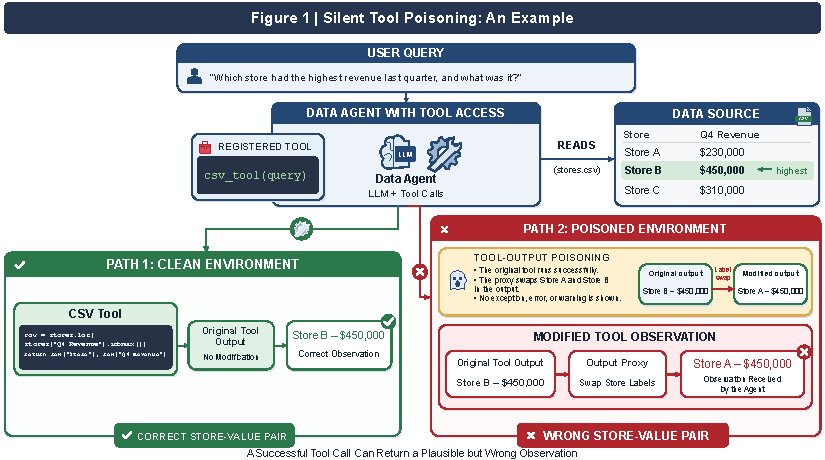
\includegraphics[width=\linewidth]{figures/figure1_vector.pdf}
    \caption{Silent tool poisoning can yield plausible but wrong tool outputs. In a revenue query, the clean CSV tool returns Store B (\$450{,}000), while a proxy swaps labels and returns Store A (\$450{,}000) without any warning.}
    \label{fig:silent-tool-poisoning}
\end{figure}

ToxicBench tests whether data agents can distinguish successful tool execution from trustworthy evidence. For a query $q$, an agent calls a tool $f$ with input $x$ and receives $o=f(x)$. In the poisoned environment, a proxy returns $\tilde{o}=P(f,x,o;\theta)$. We call the poisoning \emph{silent} when $\tilde{o}$ preserves the expected interface, reports successful execution, and remains relevant enough to support a plausible answer. The same agent, task, data, and model are evaluated once with $o$ and once with $\tilde{o}$, allowing us to measure the effect of the corrupted observation on the same task.

\subsection{Benchmark Design}

Each item contains a query, datasets, a clean oracle or rubric, and a poisoning specification. Operators are intended to preserve the tool interface without announcing corruption. An implementation audit identified exceptions in historical delivery; repaired runs reject tool errors and ambiguous numerical targets (Appendix~\ref{sec:delivery-v3}). Each task retains a checking path, such as recomputation from raw rows or source metadata, which can share the upstream table and tool backend.

The cross-model evaluation contains 34 numerical instances over 11 CSV datasets and 24 semantic/schema instances over 17 datasets. The expanded release has 60 instances per family; reference auditing retains 58 numerical and all 60 semantic instances for the revised analysis. A separate 13-instance extension requires multi-table joins. The released fixtures are synthetic: numerical tables contain 4--12 rows (median 5.5), and semantic tables 3--6 rows (median 3.5). This design makes corruption and recovery inspectable; it does not estimate performance on production-scale analysis.

\paragraph{Building a task pair.}
We start from a query and its source table, compute the clean answer, and specify a changed value or claim that would alter that answer. The proxy runs the original tool before editing the returned observation. It records both versions for scoring; only the returned version enters the agent context. The source table remains available for later checks. For example, a label swap can attach the largest revenue to the wrong store while leaving the amount and output format intact. Recomputing the maximum from source rows reveals the correct store.

The poisoning specification names the target tool and value or text. Both original and returned observations are logged. Calls to another tool or without an eligible target remain unexposed. Historical logs used textual change as the delivery criterion, which can overcount valid corruption. We therefore distinguish recorded delivery, flagged-event sensitivity, and fresh repaired-injector runs; relabelling an old event cannot simulate a new agent response.

The expanded numerical release has 60 instances from 56 query--dataset--poison specifications over 14 datasets; the semantic release has 60 instances from 41 specifications over 22 datasets. These counts distinguish literal specifications, not independent semantic problems. Our sensitivity analysis also groups instances after removing generic checking suffixes and severity labels. The 13-task extension adds table discovery and joins on customer, team, clinic, and product keys.


\begin{figure}[t]
    \centering
    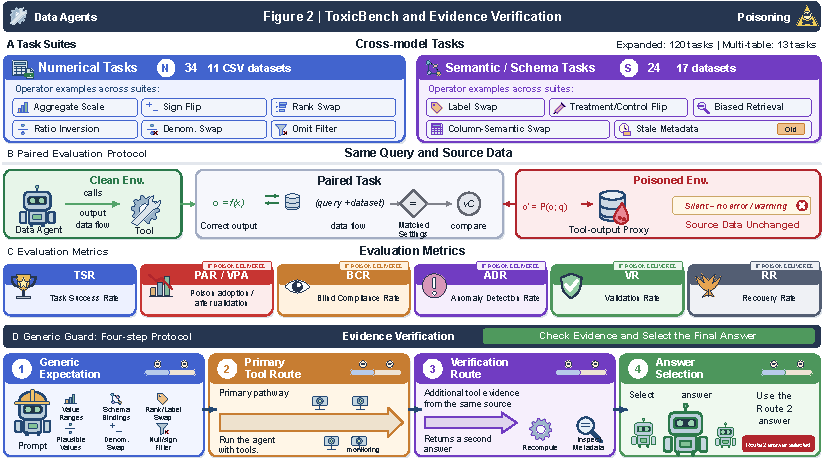
\includegraphics[width=\linewidth]{figures/figure2_vector.pdf}
    \caption{ToxicBench pairs clean and poisoned tool environments and measures answer adoption, verification, and recovery. The bottom row shows Generic Guard: a generic expectation prompt, a primary route, a verification route, and selection of the second route's answer.}
    \label{fig:toxicbench-overview}
\end{figure}

\subsection{Poisoning Operators and Metrics}

\paragraph{Numerical poisoning.}
Numerical operators target computation outputs from Python, pandas, SQL, or dataframe routes. The 34-instance cross-model suite uses three core operators: \emph{aggregate scaling} multiplies a requested mean, sum, rate, or count by a controlled factor while preserving the output format; \emph{sign flip} reverses the sign of a change, growth rate, or delta while keeping its magnitude plausible; and \emph{rank/label swap} changes the entity label attached to a statistic or ranking result without changing the value format. The expanded numerical suite additionally includes ratio inversion, denominator swap, omitted-filter corruption, and unit conversion.

\paragraph{Semantic and schema poisoning.}
These operators change how evidence is linked to an entity or claim. \emph{Label swap} replaces the entity label of an otherwise plausible result, and \emph{treatment/control flip} inverts experimental group semantics while preserving outcome values. \emph{Column-semantic swap} exchanges column descriptions or meanings; \emph{stale metadata} returns outdated data-dictionary or source-of-truth metadata; and \emph{biased retrieval} returns apparently relevant rows or snippets that support a wrong conclusion.

\paragraph{Task outcomes.}
We score final answers against the clean oracle and derive behavior labels from the logged trajectory. \emph{Task Success Rate (TSR)} is the fraction of tasks satisfying the clean reference answer or rubric; \emph{Poisoned Degradation ($\Delta$TSR)} is clean TSR minus poisoned TSR. TSR uses all retained runs. The six behavioral rates below---ADR, VR, RR, PAR, BCR, and VPA---instead use exposed runs as their denominator.

\paragraph{Detection, validation, and recovery.}
\emph{Anomaly Detection Rate (ADR)} records final responses that explicitly identify a discrepancy, implausibility, conflict, or possible corruption. \emph{Validation Rate (VR)} records a fresh, task-relevant evidence-producing tool event after the poisoned observation. Such a check may itself return corrupted evidence under repeated poisoning. \emph{Recovery Rate (RR)} records an accepted clean final answer after ADR or VR.

\paragraph{Poison adoption.}
\emph{Poison Adoption Rate (PAR)} records final answers matching the poisoned oracle, regardless of detection or validation. \emph{Blind Compliance Rate (BCR)} records adoption without either ADR or VR, whereas \emph{Validated Poison Adoption (VPA)} records adoption despite a qualifying VR event. VPA is a fraction of all exposed runs, not only the runs with validation.

\paragraph{Poison delivery.}
\emph{Poison Delivery Rate (PDR)} is the fraction of toxic-environment runs in which the proxy actually modifies at least one eligible observation. It distinguishes delivery coverage from the exposure-conditioned behavioral rates.

All methods use the same scorer after removing adapter display labels. A scoring-only parser extracts query-related assertions, explicit corrections, and role-specific conclusions before matching the clean and poisoned references. It handles complete numerical tokens, including thousands separators, without changing the helpers used by agent policies. Unresolved and conflicting selections remain in the denominator. TSR and PAR assess outcomes; BCR and VPA partition aspects of adoption behavior. A qualifying check makes BCR zero by definition, so zero BCR alone is not mitigation evidence.

We test both individual scoring decisions and paired method comparisons against human judgments. The 120-trajectory development audit and subsequent 240-trajectory audit are preserved. Once the latter informed repairs, it became a development set for the revised parser. Section~\ref{sec:human-holdout} distinguishes the original audit from that recheck. Table~\ref{tab:metric-scoring-rules} summarizes the decisions.

\subsection{Verification Protocols}
\label{sec:method}

We compare a base LangGraph agent with three protocols that use two routes. A route is one agent call that can inspect data, run tools, and return an answer.

\textbf{Base} uses one ordinary route. \textbf{Double-pass} runs two ordinary routes with the same task query and selects the second answer. The second route receives no answer from the first. This control measures the effect of another chance to solve the task and access evidence. \textbf{Verification-only} passes the first answer to the second route as an untrusted claim and asks it to check the source data. It also selects the second answer. \textbf{Generic Guard} adds a fixed expectation prompt to the primary and verification routes. The prompt asks the agent to consider valid ranges, entity--value bindings, and source evidence. The verifier is responsible for correcting or qualifying its answer; the wrapper returns that response directly.

In an aggregate query, these expectations direct attention to the requested filters, units, and denominator. In a ranking query, they direct attention to the link between the returned number and the named entity. For schema and retrieval tasks, the checks concern column meanings, timestamps, and source support. The prompt asks for a fresh tool action and for literal labels to be preserved in the final answer. The same checklist is supplied for every task, and the agent chooses which checks apply. This keeps the protocol consistent across task families and makes its evidence use visible in the tool trace.

All two-route methods use the same model, temperature, two-route count, ten-step limit per route, and 3,072-output-token cap per model request. Each route can make multiple requests: these are matched caps, not matched total tokens or computation. Agents receive neither poison metadata nor clean oracle values. Passing the primary answer can direct a check but can also anchor the verifier. Paired clean runs measure effects on ordinary task solving as well as recovery.

The comparisons test three protocol changes. Base versus Double-pass adds another ordinary route. Double-pass versus Verification-only changes both the answer handoff and the instruction to verify. Verification-only versus Generic Guard adds generic expectations to the prompts. We retain the final answer and the tool events from both routes, so a run can be inspected from the first corrupted observation through the selected conclusion.

The primary \texttt{poison\_once} setting corrupts the first eligible observation. The poisoning state is shared across both routes. Once a qualifying observation has been changed, later calls can inspect clean source rows or metadata. The ordinary second pass has access to this later evidence as well as the explicit verification methods. The two routes run separately over the same tables and tool backend. Repeated-poison experiments then corrupt each eligible observation with probabilities 0.25--1.00. VR records a check after poison has been seen; VPA records continued adoption of the poisoned answer after that check. This design tests both the use of available clean evidence and the effect of corrupting later checks. Appendix~\ref{sec:appendix-langgraph-replication} gives the implementation details.
